\documentclass[sigconf]{acmart}

\usepackage{graphicx}
\usepackage{hyperref}
\usepackage{todonotes}

\usepackage{endfloat}
\renewcommand{\efloatseparator}{\mbox{}} % no new page between figures

\usepackage{booktabs} % For formal tables

\settopmatter{printacmref=false} % Removes citation information below abstract
\renewcommand\footnotetextcopyrightpermission[1]{} % removes footnote with conference information in first column
\pagestyle{plain} % removes running headers

\newcommand{\TODO}[1]{\todo[inline]{#1}}

\begin{document}
\title{Big Data Analytics in Data Center Network Monitoring}


\author{Dhanya Mathew}
\orcid{HID328}
\affiliation{%
  \institution{Indiana University}
  \streetaddress{711 N Park Ave}
  \city{Bloomington} 
  \state{Indiana} 
  \postcode{47408}
}
\email{dhmathew@iu.edu}

% The default list of authors is too long for headers}
\renewcommand{\shortauthors}{G. v. Laszewski}


\begin{abstract}

Data Centers are evolving and adapting to newer strategies like virtualization. It is very challenging to monitor the current complex network infrastructure and its performance. Big data technologies promise solutions for network monitoring and performance analysis on real-time data. Big data streaming technologies offer high availability, high throughput, low latency and horizontally scalable solutions. Big data applications use distributed architectures and work on a huge volume of either offline data or streaming data or both. 

Network monitoring solutions monitor the infrastructure, collect generated events, stream it and analyze it using a distributed analytics platform. Insights are derived out of this analysis. These insights facilitate the authority to take data-driven decisions. Big data analytics correlates data from different sources in real-time along with historical data to identify issues proactively. This helps either an automated system or human intervention to take necessary steps before the event actually happen. We explore the various network traffic monitoring and data analytics processes involved in the networking world like fault monitoring, performance monitoring and threat analysis.

\end{abstract}

\keywords{i523, HID328, big data, fault monitoring, threat analysis, event streaming, Flink}


\maketitle



\section{Introduction}

Network administrators are mostly located remotely. Data center infrastructure monitoring and network traffic monitoring are one of the most critical parts of any enterprise. Good amount of planning should be there to choose the right monitoring solution, the set of things or events to be monitored and perform timely maintenance or upgrades of the tools \cite{how-to-monitor-and-manage-your-data-center-network}. Traditional Data Center monitoring tools can only monitor limited amount of events or thresholds. It is normally presented on a dashboard for the analyst to look on it but they could not relate the information from different sources. Often these tools gets outdated based on the high volume of data, newer technologies, data center scalability and configuration databases used \cite{how-analytics-can-help-your-customers-improve-data-center-operations}. 

A good monitoring solution needs to be able to alert you to issues with server hardware, operating system errors, application errors, networking hardware issues, and environmental issues. There is no single monitoring solution that can perform all of these functions. Hence an administrator should integrate multiple monitoring solutions to monitor different alerts and configure the alerts in such a way that it triggers email or message to the right team to take action. Als, the alerts need to be routed to a storage and analytical solution as well for further analysis. Current monitoring solutions should be able to handle virtualization challenges \cite{how-to-monitor-and-manage-your-data-center-network}. 

By applying big data to data center operations, we can analyze the statistical and performance data obtained from multiple network devices like physical servers, virtual servers, routers, switches, firewalls, access points, storage etc. Big data can provide centralized and predictive analytics and we can identify the weak points in the system and determine what changes might improve the network performance \cite{key-benefits-of-managing-data-center-operations-with-analytics}.

\begin{figure*}[htb]
  \centering
  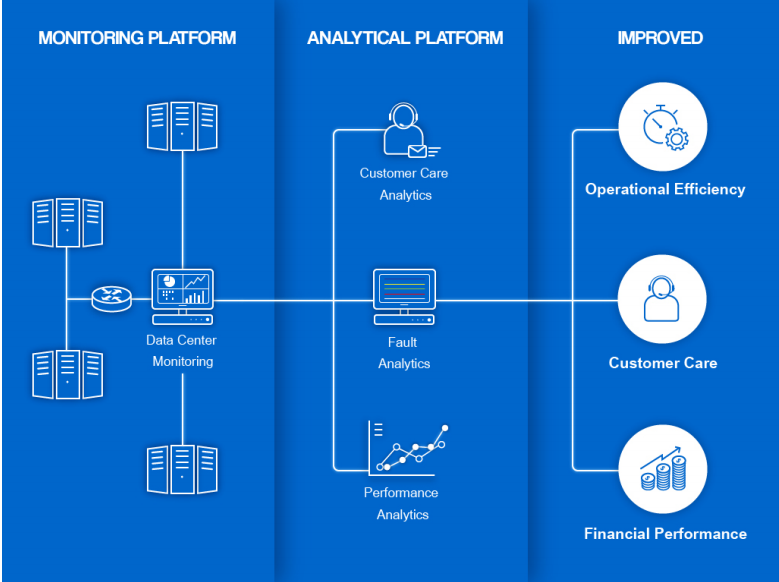
\includegraphics[width=1.0\textwidth]{images/Figure1.png}
  \caption{Monitoring and analytical platform 
  \cite{datacenter-monitoring-and-analytics-platform}}
  \label{fig:Figure1} 
\end{figure*}

As shown in Figure \ref{fig:Figure1}, data center monitoring platform is capable of monitoring all types of network devices. The events captued by the monitoring tools will be passed to the big data analytical platform for processing. Here events from different monitoring tools will be integrated and related to obtain the insights. These insights would be the base for deriving decisions and in turn results improvements in operational efficiency and financial performance etc.

\section{Data Center Network Monitoring}

There are a number of IT infrastructure monitoring tools which can be integrated with big data analytical platform. AppDynamics (Application and server performance monitoring), CopperEgg (IT Infrastructure monitoring), Datadog (Cloud monitoring), Logicmonitor (monitors networks, servers, storage and cloud), Gear5 (Website performance monitoring) are some of them \cite{top-server-monitoring-application-performance-monitoring-apm-solutions}. IT infrastructure devices vary by type and manufacturer and the alarm or events need to be monitored will also vary accordingly. Fault, performance and SLA (Service Level Agreement) monitoring are very basic level of monitoring required for all types of devices.

\subsection{Fault Monitoring}

The fundamental task of system managers is to identify and rectify the faults in the network design and architecture. As today's huge Data Centers uses cloud networks,vitualization, parallel processing, load sharing etc, it is very crucial to detect, identify and remediate the network faults. Users may be connected to the network via locally or remotely via internet technologies. Faults in any of these areas will cause customer dissatisfaction. 

Data centers are designed for scalability and hence network devices and servers are continuously get added, upgraded or replaced. Each fault that could happen in a data center can throw dozens of error reports. Hence the usage of a fault correlation software is important. This can be achieved by mechanisms like TL1 messages, SNMP traps, SYSLOG entries and application logs \cite{network-fault-management-in-todays-complex-data-centers}. The basic areas getting monitored on servers and network devices as part of fault monitoring are, server and network alarms, events, event enrichment and automatic notifications.

\subsection{Performance Monitoring}

Network performance depends on the type and capacity of the network connecting users to the application. Whenever an end user reports slow access to an application, the issue could be with the server or bandwidth or application itself \cite{network-monitoring-datacenter-management}. An event correlation software is essential here as well.

The basic areas getting monitored as part of performance monitoring are, network performance, server and network performance threshold and SLA monitoring.

\section{Data Center's Big Data Analytics}

Bringing big data analytics to data center operations and can provide data-driven insights which may not be obtained from traditional monitoring tools. Infrastructure analytics tools are bringing big data processing techniques (e.g., Hadoop, NoSQL and Cassandra) into the data center, for quicker, more informed infrastructure management decisions \cite{IT-analytics-tools-bring-big-data-to-work-in-the-data-center}.


Applications of big data are constantly growing and in turn the growth of data centers and cloud infrastructure as well. More than any of these, the number IoT devices have the most growth rate. According to Gartner Inc, by 2020, there will be 26 billion units IoT devices installed generating 44 Zetta Bytes of data in total \cite{communications-network-technology-advances}, \cite{digital-universe}.

\begin{figure}[htb]
  \centering
  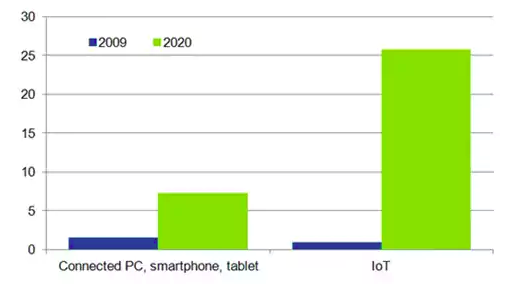
\includegraphics[width=1.0\columnwidth]{images/Figure2.png}
  \caption{Total of connected devices (in billions) 
  \cite{communications-network-technology-advances}}
  \label{fig:Figure2} 
\end{figure}

Figure \ref{fig:Figure2} shows the data generation in billions per devices types. This huge data generation by default increases the growth of data centers by adding more and more servers and network devices. Even a simple addition to the current infrastructure would require detailed monitoring in terms of compliance, security and performance.


\subsection{Server and Network Performance Data Analytics}

Traditional data center monitoring tools are developed for pre-cloud era. Today, digital applications are distributed and traditional monitoring tools may not be effective. Hence Big Data based tools are necessary. Kentik introduced a new network performance management (NPM) tool for cloud based distributed applications and data centers \cite{kentik-introduces-new-npm-solution}. Kentik's NPM solution builds on Kentik Detect, the big data-based, SaaS network analytics platform chosen by digital leaders like Yelp, Box, Neustar, Pandora and Dailymotion.

Kentik's NPM solution has a host based agent called nProbe which can be deployed in hybrid data centers and cloud networks. This could monitor and analyse network performance factors such as latency, re-transmits, out of order packets, and packet fragments based on actual application traffic flows, offering the most relevant and actionable intelligence \cite{kentik-introduces-new-npm-solution}.

\begin{figure*}[htb]
  \centering
  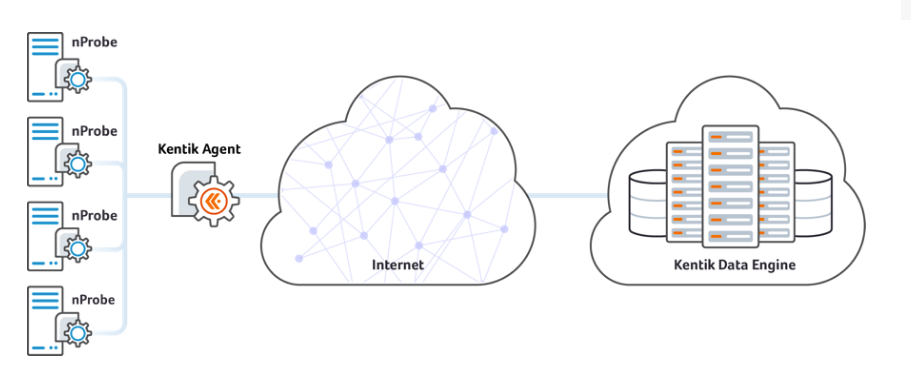
\includegraphics[width=1.0\textwidth]{images/Figure3.png}
  \caption{Big data based SaaS NPM solution 
  \cite{big-data-network-performance-monitoring}}
  \label{fig:Figure3} 
\end{figure*}

As shown in Figure \ref{fig:Figure3}, nProbe running on host computers send network performance monitoring data securely to Internet via encrypting proxy agent which is optional. Kentik data engine receives this data from internet and stores this data for actionable analytics. This data engine is big data based and can scale horizontally to store unsummarized data and provides powerful analytics for alerting, diagnostics and other use cases. Big data performance analytics may execute on performance data to, examine performance patterns, find commonalities, derive actionable insights. The actionable insights that can be derived are, identifying devices exhibiting deviation from normal pattern, predict network performance and load balancing requirements.


\subsection{Server or Network Fault Data Analytics}

In practice, historical failure data integrated with real-time data are often used to estimate the failure distribution of an item using statistical methods. This leads the way to predict future failures with a data-driven confidence level. Initially, this worked only when the particular device operated in a relatively stationary environment with no chances of changes. Given the complexity of modern systems, multiple failure mechanisms may interact with each other in a very sophisticated manner. Environmental uncertainties may also have a great impact on the occurrence of failures. This requires predicting future failures of an item based on data which can reflect its real condition. It has been estimated that 99 percent of machinery failures are preceded by some malfunction signs or indications \cite{big-data-analytics-for-fault-detection}. 

\begin{figure}[htb]
  \centering
  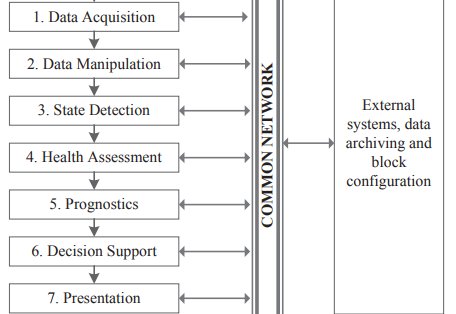
\includegraphics[width=1.0\columnwidth]{images/Figure4.png}
  \caption{Fault detection architecture 
  \cite{big-data-analytics-for-fault-detection}}
  \label{fig:Figure4} 
\end{figure}

Figure \ref{fig:Figure4}, shows the network fault analysis architecture using big data. The procedure include activities like, mine network event patterns, find commonalities, actionable insights and prediction of network Faults.

\subsection{Customer Care Data Analytics}

Another main area of consideration in data center operations is Customer care. Using big data technologies we can track the entire customer journey including their previous and following operations. In particular related to data center, it is essential to analyze customer services, support emails, call logs and trouble tickets in order to understand their network and operational behaviour. 

Based on big data classification algorithm, we can predict the customer satisfaction index and the possibility of a customer to churn out of business. Clustering algorithms are effective in predicting new customer plans and their network and infrastructure planning.

\subsection{Threat Analysis}

Network is vulnerable to cyber-attacks. Once the network is compromised, the attacker can infiltrate the enterprise and gain access to important corporate and personal data. This can cause significant damage to the business. Since an attack results in significantly above network traffic than usual, monitoring traffic for abnormal patterns can facilitate the detection of most of the cyber-attacks.

A well designed threat detection system consists of network data collector, streaming module (Kafka, Storm etc.) and Analysis module. Collector will collect the data from network and send the data to Streaming module. Then the stream will be sent to analysis module. Analysis module consists of the latest streaming analysis technologies (Flink, Spark Streaming etc.) and the threat detection mechanisms to detect malicious activities. Cloud environment will give the advantage of concurrently processing huge volume of data and also increase the efficiency of monitoring and threat detection process.  

Instead of offline analysis, we can utilize the statistical tools to extract meanings and use these models in the streaming data analysis to detect the threat. Statistical model may become more accurate as volume of data increases and can adapt to changes in the data over time. All these things should happen without compromising the time complexity and efficiency. We can use streaming k-means clustering algorithm and Fuzzy c-means clustering algorithm both of which can identify patterns over time to make the accurate decision \cite{streaming-based-network-monitoring-and-threat-detection-system}.

In the below example of threat detection system, a test server is used with ports open for the experimental purpose. The system was trained with normal traffic data with around the size of 260 GB in pcap format containing network traffic packet information. 

\begin{figure}[htb]
  \centering
  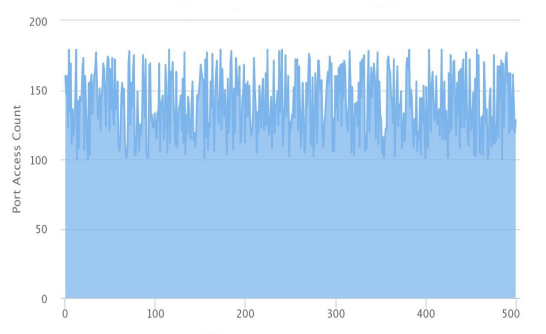
\includegraphics[width=1.0\columnwidth]{images/Figure5.png}
  \caption{Ports access count within range 100 to 180 per minute
  \cite{streaming-based-network-monitoring-and-threat-detection-system}}
  \label{fig:Figure5} 
\end{figure}


\begin{figure}[htb]
  \centering
  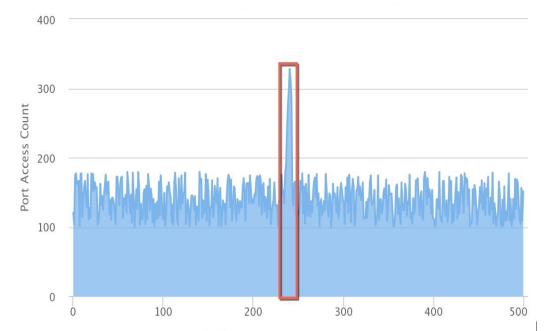
\includegraphics[width=1.0\columnwidth]{images/Figure6.png}
  \caption{Ports access count shows abnormal port activity
  \cite{streaming-based-network-monitoring-and-threat-detection-system}}
  \label{fig:Figure6} 
\end{figure}

Figure \ref{fig:Figure5} shows that the port access count is within the range of 100 to 180 per minute. In figure \ref{fig:Figure6}, it clearly indicates that there is some abnormal activities happened in between time 220 to 245 \cite{streaming-based-network-monitoring-and-threat-detection-system}. Administrators will be triggered for any such kind of activities immediately. 


\section{Improvements}

Having big data in data center operations results improvements in \cite{datacenter-monitoring-and-analytics-platform},

\begin{itemize}
\item Operational efficiency
\item Reduce infrastructure/network down time
\item Improve customer experience
\item Financial performance
\item Reduce network/infrastructure operations expenditure
\item Reduce customer churn
\end{itemize}


\section{Conclusion}

Today's networks pose performance and security challenges to network managers because of the layers of redundancy, management and virtualization. The only practical approach for the networking team is to stream or collect all the network related data which is voluminous and varied, into an analytical framework. Big Data analysis is opening up new sales opportunities and risk alleviation in the networking world. Organizations are already benefiting increased uptime, faster troubleshooting and improvement in security by on-boarding Big Data analytics in the network infrastructure.

\begin{acks}

The author would like to thank the web loaded with information. The author would also like to thank Prof. Gregor von Laszewski for his guidance and suggestions.

\end{acks}

\bibliographystyle{ACM-Reference-Format}
\bibliography{report} 




\end{document}
